\vspace{-5pt}
\section{Implementation}
In this section, we outline the processes of preparing the tools we used in our study, including the survey elements of the pre-app task and post-app task, as well as the app itself.
\vspace{-5pt}
\subsection{Development of the App}
The app was created using the visual programming interface, MIT App Inventor 2, version nb185a, and exported as a Android Package Kit (APK) using MIT App Inventor Code, version code36. An APK is a file format used by Android to distribute and install apps. The app was programmed to collect detailed logs of users' interactions (e.g., clicks, time-stamps) to assist in identifying user behavior and level of interaction. 


This app begins by presenting monster avatars that each have an associated macronutrient goal. In each round users are shown four meal photos and are asked to pick which one best fits their monster's goal then to type in a short reason why they selected that meal for their avatar. Once a meal photo is selected, users are taken to a community board (CB) to see what others decided. Each user has the option of changing their mind or moving forward with their original selection. Once more the user types in the reason for sticking to their choice or changing their meal. Once a meal photo is selected the round is over. There are a total of five rounds. The app also randomized the meal choices within each round, as well as the order of the rounds themselves. App components are further described in more detail below (see Figure~\ref{fig:screenshots}).



\begin{figure}[!ht]
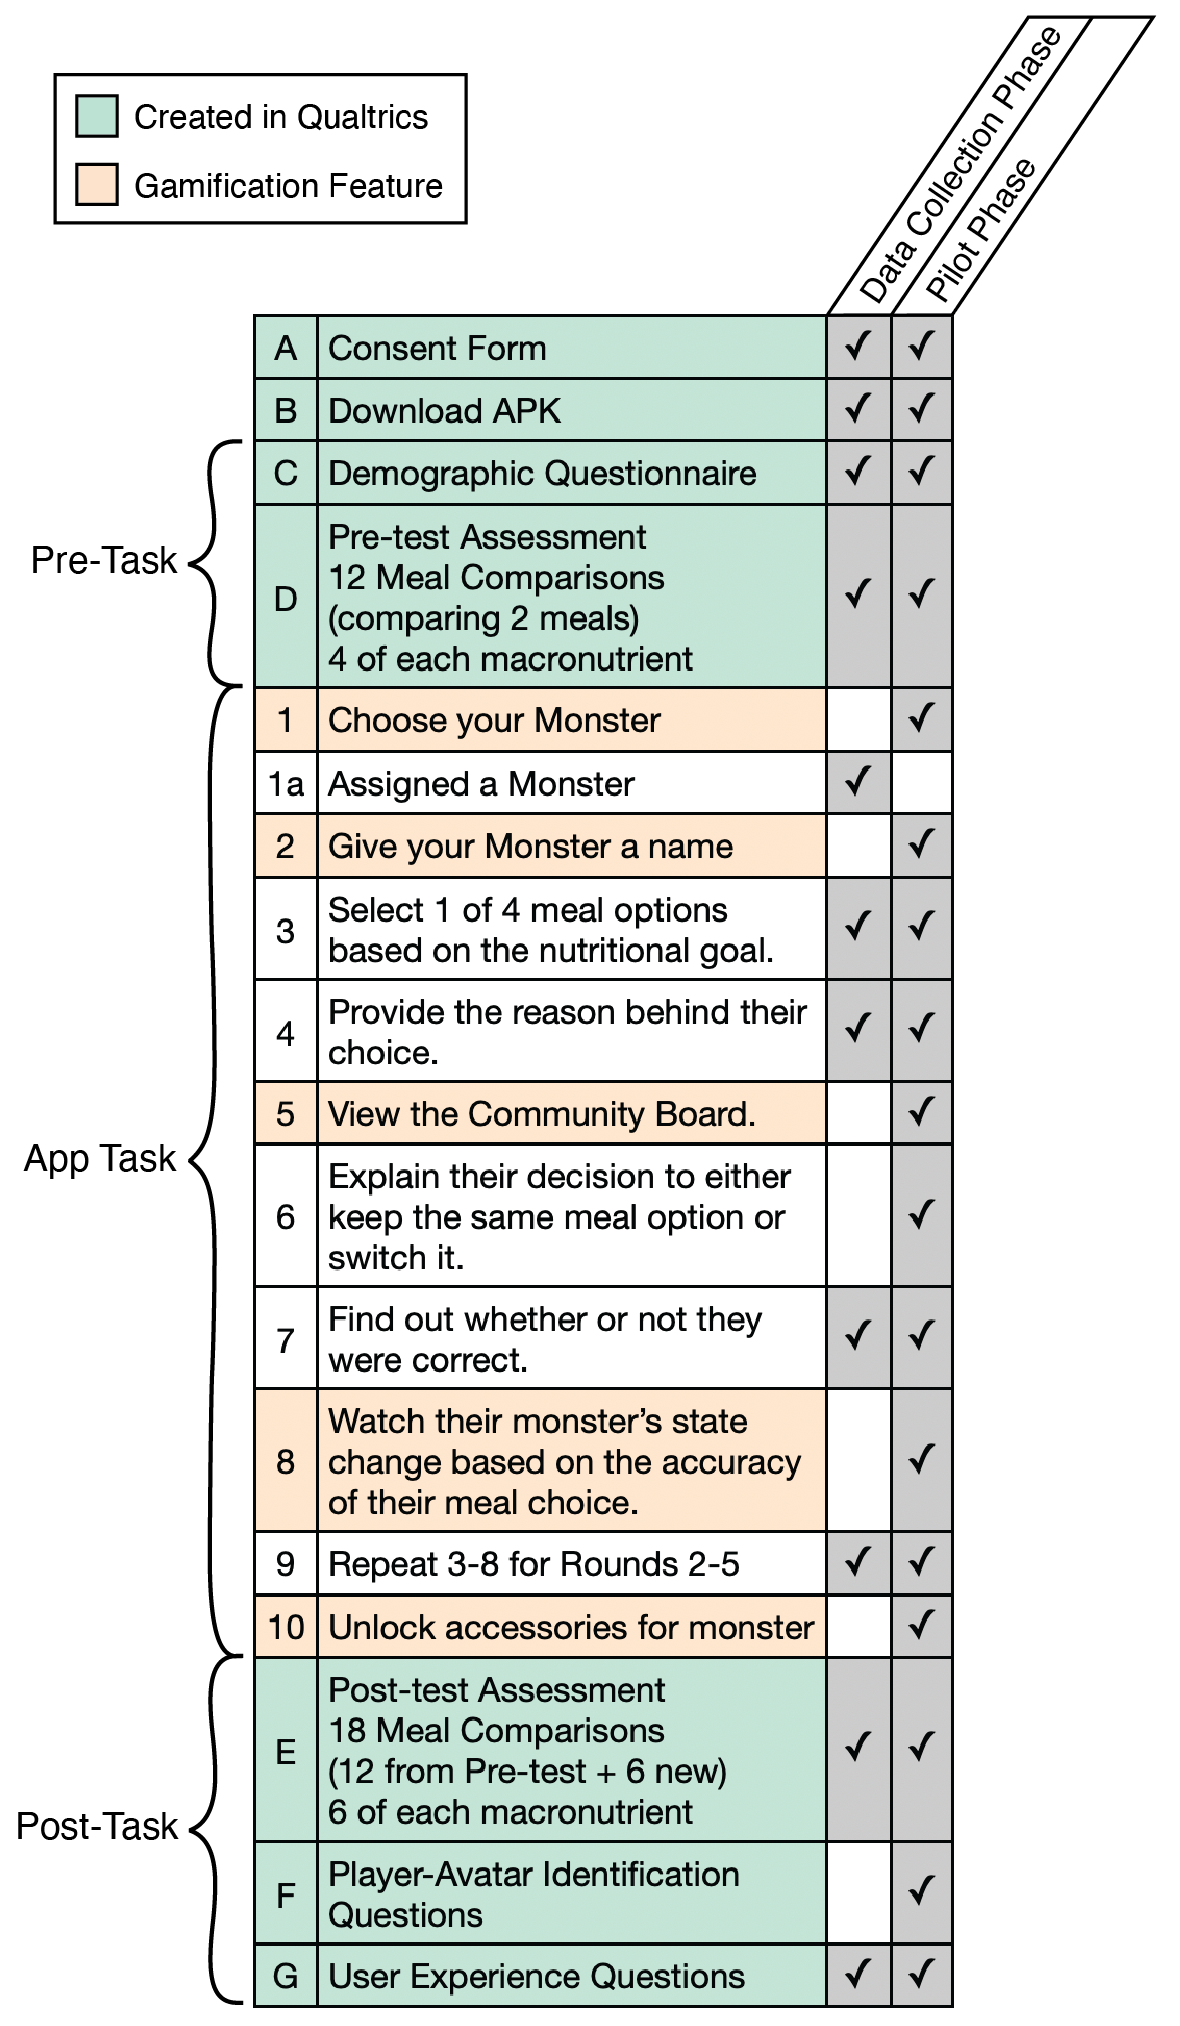
\includegraphics[scale=0.33]{samples/images/figure-2-02.png}
\caption{Chart showing the steps of the study and the differences between the Data Collection Phase and Pilot Phase.}
%\vspace{-15pt}
\label{fig:phasechart}
\end{figure}
%\setlength{\textfloatsep}{3pt plus 1.0pt minus 2.0pt}


\begin{figure}[!ht]
\includegraphics[width=\textwidth]{samples/images/screenshots2.png}
\caption{Series of screenshots showing the main steps of the app. Pilot Phase only. }
\label{fig:screenshots}
\end{figure}


\vspace{-5pt}
\subsection{Gamification Mechanisms for the App}
\subsubsection{The Ability for the User to Select and Name a Pet Monster Avatar} 
There are four monsters in the app, each with their own brief background story as to why they are pursuing their nutritional goal. 
For example, one monster's story reads: \textit{``This monster has Irritable Bowel Syndrome. Their daily life is greatly influenced by the way their digestive system behaves. One part of their treatment plan is managing their diet. Their dietitian has given them the goal of increasing the amount of fiber in their diet''}. 

In the Data Collection Phase (DCP), participants were assigned to their pet monster avatar and provided with its story and corresponding nutritional goal. In the Pilot Phase (PP), users could choose their own monster avatar with a corresponding health goal. After selecting one of the four monsters, users were asked to give their monster a name. 
This custom name was used throughout the rest of the app. Figure~\ref{fig:screenshots} shows screenshots of the flow.


\vspace{-5pt}
\subsubsection{Viewing the Community Board (CB) of Crowdsourced Intelligence}

The inclusion of a CB made input from the crowd available to assist the user in deciding which meal best fits the chosen nutritional goal. 
The CB displayed both the percentage of the crowd that selected each of the four meal options and three user-generated reasons explaining why users chose that meal option. The user-generated reasons presented in the pilot were collected in the DCP. 




\vspace{-5pt}
\subsubsection{Monster's State Change and  Unlocking Accessories} 

After users viewed the CB and submitted their final meal choice,
%with a text-based reason, 
they were able to watch their pet monster avatar react to the meal they chose to feed them. 
If the monster was fed the best choice meal for their nutritional goal, the user saw their monster avatar's physical state improve in a short animated morph. If the monster was given the second best meal, their condition remained unchanged. 
If the user fed their pet monster either of the two worst options, they saw its physical state degrade in the animated morph. If within the five meal rounds, a user answered four or more questions with the best meal option, the user unlocked the accessories screen, where they were able to choose one of four accessories to award their pet monster as shown in Figure~\ref{fig:monster-stages}. 
Given the five rounds, users could win up to two accessories.

\begin{figure}[h]
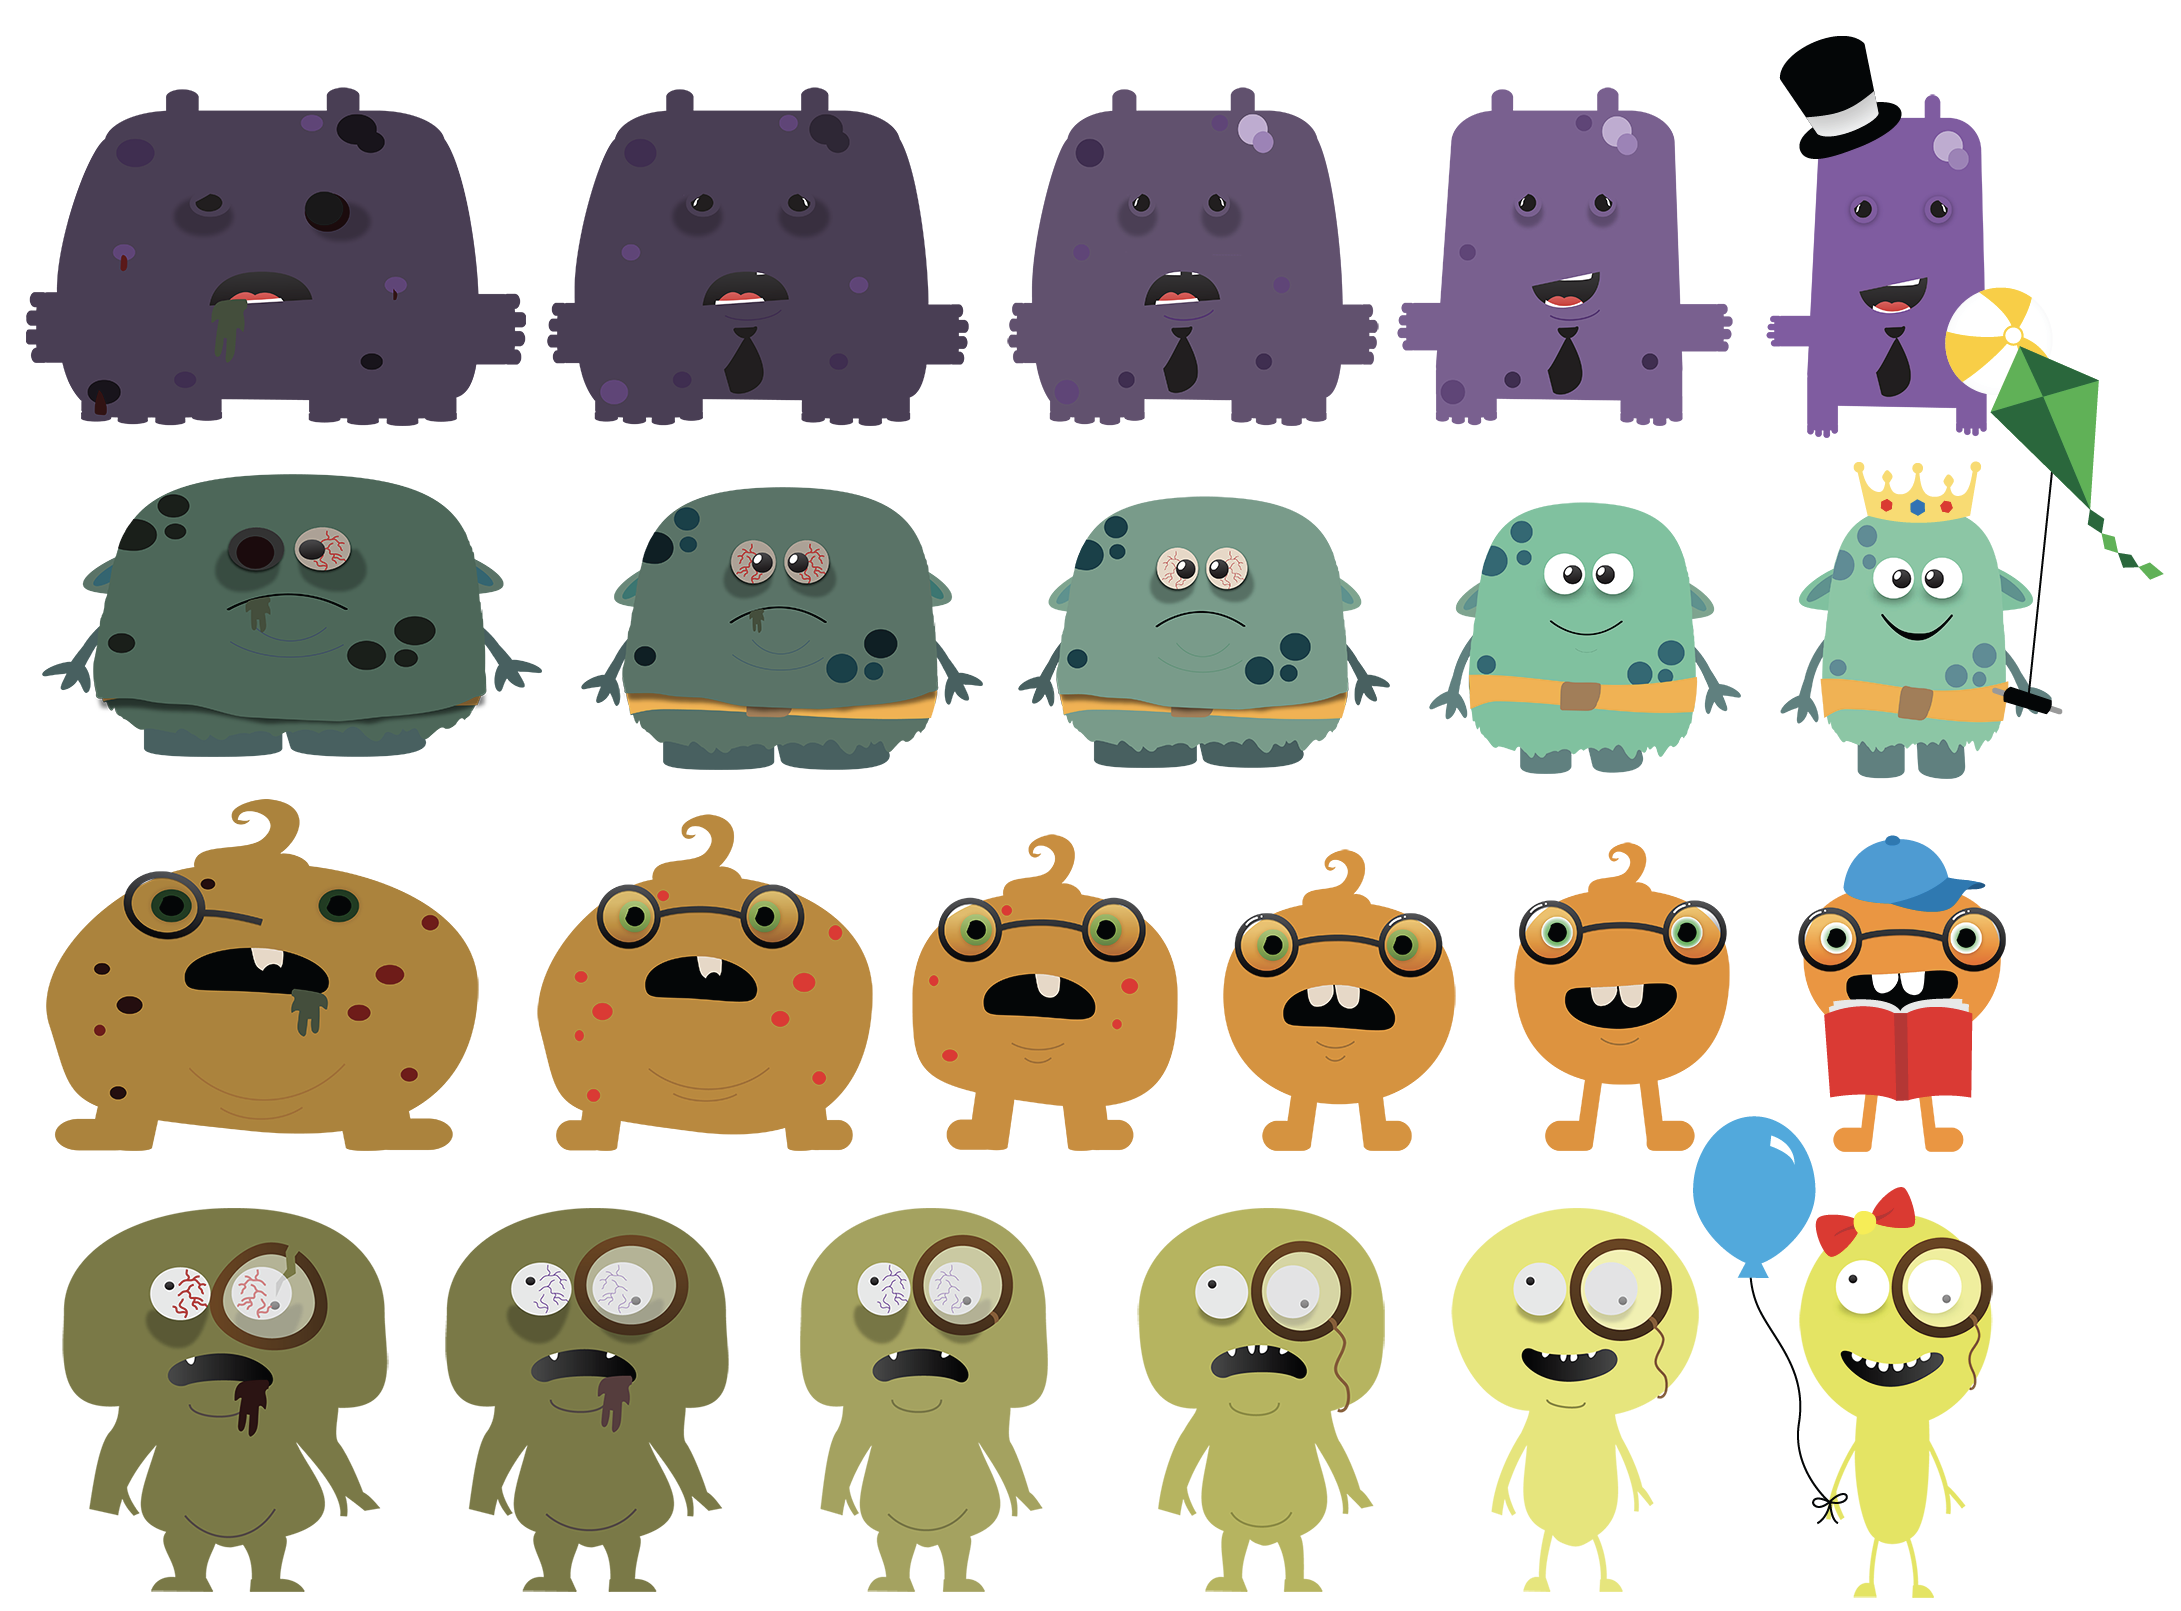
\includegraphics[scale=0.25]{samples/images/figure-5.png}
\caption{Sample of various monster condition stages. Monsters started in the middle, ``Neutral,'' and became ``Less Healthy'' (left) or ``More Healthy'' depending on user's meal choices. The far right shows avatars with the available accessories when unlocked.}
\label{fig:monster-stages}
\end{figure}



\vspace{-5pt}
\subsection{Development of Surveys}
There were two pre-task surveys: 1) a demographic questionnaire, and 2) pre-test nutritional assessment.
In the demographic questionnaire, users were asked basic demographic questions and questions about their prior experiences with nutritional knowledge and health related apps. The pre-test nutritional assessment consisted of 12 questions in which users were tasked with identifying which of two meal options better fit a given macronutrient content goal (e.g., which meal photograph is higher in carbohydrates). 
Participants did not receive feedback on the accuracy of their responses. 
There were four questions for each macronutrient type (i.e., carbs, fat, fiber). 

The post-task consisted of three surveys: 1) the post-test assessment, 2) player-avatar-identification (PAID) questions, and 3) user experience questions.
The 18 question post-test assessment was similar to the pre-test assessment and also asked the user to identify which of two meal options better fit for the given macronutrient goal.
The 18 meal identification questions consisted of six questions for each of the three macronutrient types. For each macronutrient type, four of the six questions contained meals repeated from the pre-test assessment, with the remaining two questions based on new meals. No meals from the app were used in the pre- and post-test assessments. Participants did not receive feedback on the accuracy of their responses. 

The PAID questions were adapted from the previously validated Player-Avatar Identification Scale~\cite{li2013player}. %using a 5-point Likert scale. 
The user experience questions focused on why users chose their monster, since users were able to select their pet avatar. The consent form, demographic questionnaire, pre-test assessment, post-test assessment, player-avatar identification questions, and the user experience questions were all created and collected using the online survey platform, Qualtrics.

\vspace{-5pt}
\subsection{Meal Photo Selection}
The app features 37 photographs of ``in-the-wild'' meals, and the pre- and post-test assessments used an additional 36.
The 73 total meal photographs were gathered from the researchers' prior studies
%~\cite{desai2019personal,mitchell2019wish} 
that used professional dietitians to complete the expert nutritional assessments. We filtered the images based on their resolution quality and content clarity, so that users were able to easily identify the components of the meals.

In each of the five rounds of the app, users were presented with four ``in-the-wild'' meal photographs, each accompanied by a brief description of its contents (e.g., Fat free Greek yogurt with grapes and coffee). We created the rounds so that each had three types of outcomes: one best choice, one second best choice, and two equally less desirable choices, ranked as such by their macronutrient content assessment. We tested the accuracy of the meal choice rankings by circulating all rounds to nutrition experts. 
We then adjusted the questions as necessary to achieve above 50\% expert agreement for all rounds and assessments. 

In the pre- and post-test assessments, each question compared two ``in-the-wild'' meal photographs, with only one being the correct option, and the other being incorrect.
